\documentclass[11pt]{article}
\usepackage[utf8]{inputenc}
\usepackage[T1]{fontenc}

\usepackage[margin=1in]{geometry}
\usepackage{graphicx}
\usepackage{booktabs}
\usepackage{amsmath}
\usepackage{amssymb}
\usepackage{caption}
\usepackage{subcaption}
\usepackage[expansion=false]{microtype}
\usepackage[hidelinks]{hyperref}
\usepackage{xcolor}
\usepackage{titlesec}
\titleformat{\section}{\normalfont\large\bfseries}{\thesection}{0.6em}{}
\titleformat{\subsection}{\normalfont\normalsize\bfseries}{\thesubsection}{0.6em}{}

\graphicspath{{./}{figs/}}
\captionsetup{font=small,labelfont=bf}

\title{\bfseries An Independent Angular-Statistics Test for\\
Crystallographically Forbidden Symmetry in the\\
Darb-i Imam Girih Tiling}
\author{Scott Cundill\\
\small Independent Researcher, Okinawa, Japan\\
\small scott.cam@gmail.com}
\date{Technical Note, June 2026\\
\small DOI: \href{https://doi.org/10.5281/zenodo.20603223}{10.5281/zenodo.20603223}}

\begin{document}
\maketitle

\begin{abstract}
\noindent
Lu and Steinhardt (2007) showed that the girih tiling on the Darb-i Imam shrine
(Isfahan, 1453 C.E.) is a nearly perfect quasicrystalline pattern, with
crystallographically forbidden ten-fold orientational order, by mapping the
tiling onto Penrose tiles and demonstrating quasi-periodic translational order.
We ask a narrower, independent question by a completely different route. If the
tile arrangement carries forbidden orientational symmetry, that symmetry should
be visible in the angular statistics of the tile centroids alone, with no
tile-to-Penrose mapping and no appeal to translational order. We extract tile
centroids from an image, treat them as a point cloud, and measure the strength
of $n$-fold rotational symmetry in the nearest-neighbour angular distribution.
The discriminator is a single scalar, the forbidden excess, defined as the
stronger of the five- and ten-fold signals minus the stronger of the four- and
six-fold signals. It is positive for quasicrystalline arrangement and negative
for periodic arrangement. The measurement is performed with an existing
open-source instrument, SCOTT (Structural and Coherent Order in Topological
Transforms), used here without domain-specific tuning. Against a calibrated set
of synthetic controls, a Penrose tiling reads $+1.14$, two genuinely periodic
tilings read $-7.81$ (square, four-fold) and $-3.77$ (hexagonal, six-fold), and
white noise gives a trivial null. A girih reconstruction of the Darb-i Imam
small-scale pattern reads $+1.29$ (full image at native aspect ratio, 406
motifs), on the quasicrystalline side with Penrose and far from both periodic
controls. The result is an independent corroboration, by
orientational statistics, of the forbidden symmetry Lu and Steinhardt identified.
It is a screening test, not a constructive proof, and it is applied here to the
authors' reconstruction as an instrument check. A test on a photograph of the
shrine wall itself is the natural next step and is not attempted here.
\end{abstract}

\section{Introduction}

The conventional account of girih patterns in medieval Islamic architecture
held that they were drafted as networks of zigzagging lines with straightedge
and compass. Lu and Steinhardt \cite{lu2007} showed that by 1200 C.E. these
patterns were being constructed instead as tessellations of a small set of
decorated polygons, the girih tiles, and that by the fifteenth century the
approach was combined with self-similar subdivision to produce nearly perfect
quasi-crystalline tilings. Their central example is the Darb-i Imam shrine in
Isfahan (1453 C.E.). They established its quasicrystalline character by mapping
the girih tiling onto Penrose kites and darts, showing the mapping is consistent
across the pattern with only a handful of point defects, and arguing that the
ratio of tile frequencies approaches the golden ratio, the signature of
quasi-periodic translational order.

A quasicrystal has two linked properties, quasi-periodic translational order and
crystallographically forbidden orientational symmetry. Periodic crystals are
limited to two, three, four, and six-fold rotational symmetry. Five-fold and
ten-fold are forbidden in a periodic tiling, and their presence in a long-range
ordered pattern is the hallmark of a quasicrystal. Lu and Steinhardt's argument
runs primarily through translational order, the Penrose mapping and the golden
ratio of tile frequencies.

We test the other property, the forbidden orientational symmetry, by an
independent route that touches neither the Penrose mapping nor the translational
argument. If the tile arrangement carries ten-fold orientational order, that
order is a property of where the tiles sit relative to one another. It should
therefore be measurable from the tile centroids alone, as an angular statistic,
with no knowledge of the tile shapes, the decoration, the Penrose
correspondence, or the subdivision rule. This is a deliberately weaker and more
local probe than the original analysis. It cannot establish quasi-periodicity,
and it does not try to. What it can do is ask whether the forbidden symmetry is
present in the raw arrangement, by a method with no overlap with the original,
so that agreement constitutes genuine corroboration rather than a re-derivation.

The measurement is carried out with SCOTT (Structural and Coherent Order in
Topological Transforms), an open-source image-analysis instrument applied in
companion work to optical bokeh \cite{bokeh}, natural and synthetic images under
amplitude-adjusted surrogate testing \cite{iaaft}, and real and synthetic faces
\cite{bilateral}. The instrument is the tool, not the subject. The contribution
of this note is the independent angular-statistics route and its calibration,
not the software that runs it.

\section{Method}

\subsection{From image to point cloud}

The input is a greyscale image. Because the discriminator measures exact angles
between tile centroids, the normalisation must preserve those angles. We
therefore pad each image to a centred square with a constant fill equal to the
image median, then downscale isotropically to a fixed $512 \times 512$ grid. The
fixed grid makes motif counts and angular statistics comparable across inputs
regardless of original size, and the pad-then-downscale order ensures the resize
is isotropic, so a genuine $n$-fold angle in the source is not deformed. The
median fill avoids injecting an artificial dark border that the extraction step
could mistake for structure. The synthetic controls are generated square, so for
them the padding is a no-op; it matters for the non-square reconstruction image,
where an anisotropic stretch would otherwise bend the very angles being
measured. The same path is applied to every specimen and control in this study.

Tile centroids are extracted by a deliberately simple pipeline. An Otsu
threshold separates bright tile interiors from dark borders. A single iteration
of $3 \times 3$ elliptical erosion separates touching tiles. Connected
components are labelled, and a centroid is taken for each component whose area
falls in the range 60 to 7000 pixels, with a relaxed fallback range applied if
fewer than fifteen motifs survive the first pass. The result is a set of
two-dimensional points, one per tile, carrying no information about tile shape,
colour, or decoration. The analysis below sees only these points.

\subsection{Angular symmetry of the point cloud}

For each point we compute the angles to its six nearest neighbours, pooled
across the whole cloud into a histogram of 72 bins of five degrees each. Five
degrees divides evenly into the $36^\circ$ spacing of ten-fold symmetry and the
$72^\circ$ of five-fold, so the expected peaks fall on exact bin centres rather
than straddling boundaries. A
pattern with genuine $n$-fold orientational symmetry concentrates angular mass
at multiples of $360/n$ degrees. We measure the strength of $n$-fold symmetry as
the mean histogram density in the $n$ exact bins at those expected angles,
expressed as an excess over the uniform baseline,
\begin{equation}
S_n = \max\!\left(0,\; \frac{\bar{p}_{\text{peak}} - 1/B}{1/B}\right),
\end{equation}
where $\bar{p}_{\text{peak}}$ is the mean normalised density in the $n$ target
bins and $B = 72$ is the bin count. The angle to a neighbour at row-column
offset $(\Delta r, \Delta c)$ is taken as $\operatorname{atan2}(\Delta c, \Delta
r)$. The measurement uses the single exact bin at each expected angle, with no
tolerance window. It is local, computed per point and pooled, so it is
insensitive to the global image boundary in a way a whole-image Fourier method
is not.

\subsection{The discriminator}

The quantity that separates quasicrystalline from periodic arrangement is the
forbidden excess,
\begin{equation}
E = \max(S_5, S_{10}) - \max(S_4, S_6).
\end{equation}
The forbidden orders five and ten are the quasicrystalline signature. The
allowed orders four and six are the periodic signature. A positive $E$ means the
forbidden signal dominates, the arrangement is quasicrystal-like. A negative $E$
means an allowed periodicity dominates, the arrangement is an ordinary crystal.
A minimum of fifteen motifs is required for any reading, and angular statistics
degrade below roughly thirty motifs, so motif count is reported alongside every
result. The excess is a simple linear difference of measured angular signals,
with no fitting, no training, and no free parameters, which keeps the
discriminator interpretable and its behaviour traceable to the geometry it
measures.

\section{Controls}

The discriminator is only meaningful if it reads strongly positive on a known
quasicrystal, strongly negative on known periodic tilings, and null on
structureless input. We locked the acceptance criteria before running the
controls. A positive control must read $S_{10} \geq 1.5$ and $E > 0$. Each
periodic negative control must produce at least 100 motifs and read $E \leq 0$.
All controls are synthetic, generated from known geometry, so the ground truth
is not in question. All run through the identical pipeline described above.

\subsection{Positive control, Penrose}

A Penrose rhombus tiling, generated by de Bruijn pentagrid dualisation, is the
canonical two-dimensional quasicrystal with exact five-fold symmetry. It reads
$S_{10} = 2.16$, $S_5 = 2.14$, and $E = +1.14$, clearing the locked gate. This
reproduces across two independent sessions on different machine builds to three
decimal places.

\subsection{Negative controls, two periodic tilings}

A genuinely periodic tiling cannot carry five- or ten-fold order, so it must
read $E \leq 0$. We use two independent periodic geometries to test both
crystallographically allowed symmetries, not just one. The first is a square
lattice of flat tiles, which carries four-fold symmetry. It reads $S_4 = 8.78$
dominating, with $E = -7.81$. The second is a hexagonal lattice, which carries
six-fold symmetry. It reads $S_6 = 4.22$ elevated, with $E = -3.77$. Both clear
the locked acceptance. The instrument does not merely register "periodic," it
identifies which allowed symmetry is present, the square control reading four-
fold dominant and the hexagonal control reading six-fold strong.

Both periodic controls are rendered in the same flat two-tone style as the
Penrose control and the reconstruction specimen, so every input is the same
visual class and extracts in the same way. This matters for the following
reason.

\subsection{A note on the surrogate that did not work}

The natural first choice for a negative control was an iterative amplitude-
adjusted Fourier transform (IAAFT) surrogate of the specimen, a randomisation
that preserves the power spectrum and the intensity distribution while
destroying spatial phase structure, used successfully on continuous-tone images
in companion work \cite{iaaft}. On a flat-colour tiling it failed, and the
failure is instructive. A flat tiling has a near-discrete intensity histogram,
so the surrogate returns speckle that the Otsu extraction cannot resolve into
tiles. The motif count collapsed from several hundred to twenty-nine, and the
power spectrum was not in fact preserved, so the surrogate was not a valid IAAFT
surrogate in the first place. We report this because it explains why the
periodic controls above, matched to the specimen's visual class and extraction
behaviour, are the appropriate negative controls for this class of image, and
because the failed surrogate is part of the honest record. Figure~\ref{fig:specimens}
shows a failed surrogate alongside the working inputs.

\begin{figure}[t]
\centering
\begin{subfigure}{0.19\textwidth}
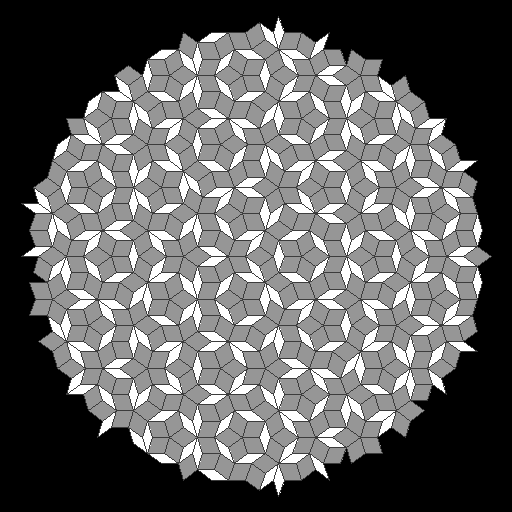
\includegraphics[width=\linewidth]{fig_penrose.png}
\caption{Penrose, $E=+1.14$}
\end{subfigure}\hfill
\begin{subfigure}{0.19\textwidth}
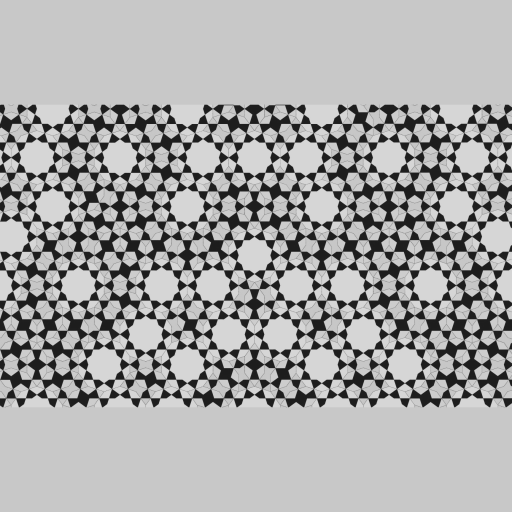
\includegraphics[width=\linewidth]{fig_recon.png}
\caption{Reconstruction, $E=+1.29$}
\end{subfigure}\hfill
\begin{subfigure}{0.19\textwidth}
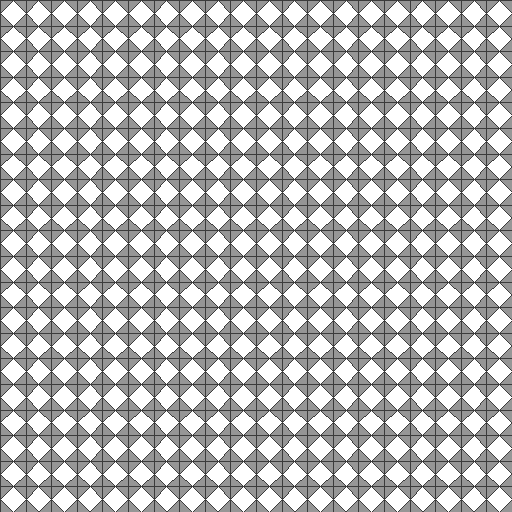
\includegraphics[width=\linewidth]{fig_square.png}
\caption{Square, $E=-7.81$}
\end{subfigure}\hfill
\begin{subfigure}{0.19\textwidth}
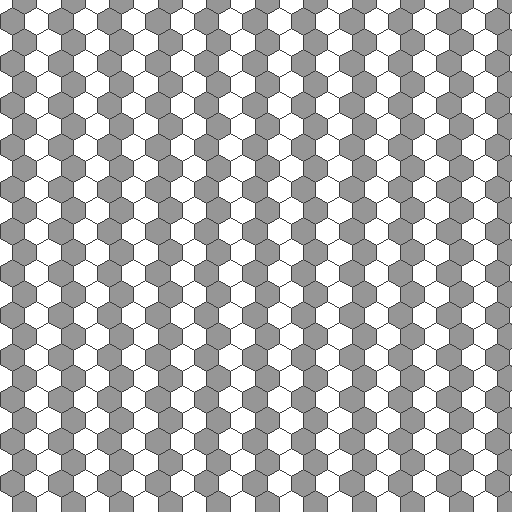
\includegraphics[width=\linewidth]{fig_hex.png}
\caption{Hexagonal, $E=-3.77$}
\end{subfigure}\hfill
\begin{subfigure}{0.19\textwidth}
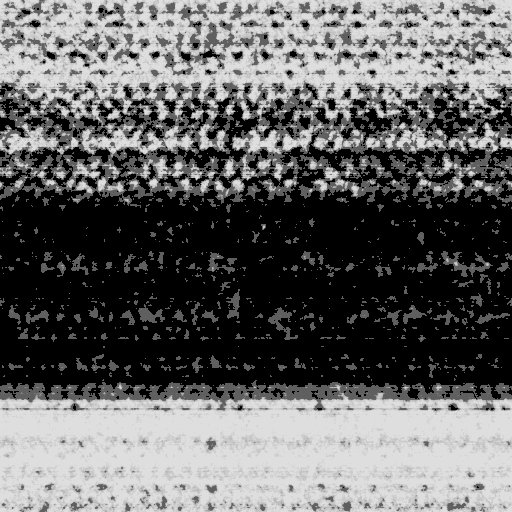
\includegraphics[width=\linewidth]{fig_iaaft.png}
\caption{Failed IAAFT}
\end{subfigure}
\caption{Inputs as the pipeline sees them, in greyscale at $512\times512$ after
padding to square. All four working specimens (a--d) are flat two-tone tilings
rendered in the same style so that extraction behaviour is matched. The two
quasicrystalline inputs (a, b) and the two periodic controls (c, d) extract
cleanly. The IAAFT surrogate (e) returns speckle that cannot be extracted, which
is why a matched periodic tiling, not a surrogate, is the appropriate negative
control here.}
\label{fig:specimens}
\end{figure}

\section{Result on the Darb-i Imam reconstruction}

We ran the test on a girih reconstruction of the small-scale Darb-i Imam pattern,
the tile pattern of Lu and Steinhardt's Figure S7A rendered in flat colour. The
reconstruction is the authors' own drawing, so this is explicitly an instrument
check, a test of whether the method reads a known quasicrystalline arrangement
correctly, not independent evidence about the shrine. The full image, padded to
square and normalised to $512 \times 512$, yields 406 extracted motifs and reads
$S_{10} = 1.71$, $S_5 = 1.73$, $E = +1.29$. The ten-fold signal clears the gate,
and the forbidden excess lands on the quasicrystalline side, above the Penrose
value and far from both periodic controls.

\begin{table}[t]
\centering
\small
\caption{Forbidden excess $E$ separates three arrangement classes on one axis.
All values from a single machine, identical pipeline. Positive $E$ is
quasicrystalline, negative is periodic.}
\label{tab:results}
\begin{tabular}{lrrrrrr}
\toprule
Specimen & Role & Motifs & $S_{10}$ & $S_4$ & $S_6$ & $E$ \\
\midrule
Penrose & positive (quasicrystal) & 671 & 2.16 & 1.02 & 0.08 & $+1.14$ \\
Darb-i Imam reconstruction & instrument check & 406 & 1.71 & 0.43 & 0.17 & $+1.29$ \\
Hexagonal tiling & negative (periodic, 6-fold) & 263 & 1.21 & 4.98 & 4.22 & $-3.77$ \\
Square tiling & negative (periodic, 4-fold) & 400 & 0.95 & 8.78 & 2.23 & $-7.81$ \\
White noise & null & 0 & --- & --- & --- & 0.00 \\
\bottomrule
\end{tabular}
\end{table}

Table~\ref{tab:results} gives the full picture. The reconstruction and the
Penrose control sit together on the quasicrystalline side of zero. The two
periodic controls sit far on the crystalline side, via different allowed
symmetries. White noise extracts no motifs and returns the trivial null. Every
populated input is a flat tiling that extracts into hundreds of motifs, so the
arrangement of the tiles is the only variable that differs between them, and the
forbidden excess separates them cleanly.

\section{Discussion}

\subsection{What this corroborates, and what it does not}

The measurement supports one specific part of the Lu and Steinhardt result, the
presence of crystallographically forbidden orientational symmetry in the tile
arrangement, by a route that shares nothing with the original argument. It uses
no Penrose mapping, no tile-frequency ratio, no subdivision rule, and no appeal
to translational order. It reads only the angular relationships between
neighbouring tile centroids. That a method with no overlap reaches the same
qualitative conclusion is the substance of the corroboration.

The method does not establish quasi-periodicity, which is the harder and more
important half of the quasicrystal definition. Forbidden orientational symmetry
is necessary but not sufficient for a quasicrystal. Forbidden orientational
order across a finite patch is noteworthy in its own right, but it does not by
itself establish aperiodic long-range order, which is the harder claim. The translational argument in the original paper remains the
load-bearing one for that claim. This note adds an independent check on the
orientational half, nothing more.

\subsection{Strength is sensitive to framing and scale}

The ten-fold reading on the reconstruction, 1.71, is below the synthetic Penrose
value of 2.16, but the forbidden excess is slightly higher, 1.29 against 1.14,
because the reconstruction's four- and six-fold content is low, so the excess
reflects the separation between forbidden and allowed signals rather than the
absolute strength of the forbidden signal. Earlier framings of the same pattern,
and the earlier anisotropic-resize pipeline, read lower on the excess, between
0.46 and 1.22, depending on how much of the pattern the crop captured and how
the normalisation set the tile scale. We also tested whether a tighter sub-crop
would sharpen the reading. It did not. A sub-crop is downscaled harder by the
fixed $512 \times 512$ grid, dropping the tile spacing below the extraction
sweet spot, the motif count fell to 192 and the ten-fold signal weakened,
although the forbidden excess remained faintly positive, the correct sign. The
full image at its native aspect ratio, padded to square, is the appropriate
input, and is the value reported above. The dependence on framing and scale is a
real limitation of a motif-extraction method and is stated plainly rather than
tuned away.

\subsection{The photograph is the real test}

The strongest version of this test is not the authors' reconstruction but a
photograph of the shrine wall itself. A photograph carries perspective skew,
uneven lighting, surface wear, and decoration laid over the tile boundaries, any
of which can defeat the extraction step. We have not attempted it here. When we
do, the pre-registered protocol is to set all preprocessing parameters on the
reconstruction, where the answer is known, then apply them unchanged to the
photograph, to run the identical pipeline on a periodic control which must stay
negative, and to disclose every preprocessing step with before and after images.
If the photograph reads positive under that protocol, it would be independent
evidence about the shrine. If it does not, that is an acceptable and reportable
limit of a motif-extraction method on worn architectural photography, and the
corroboration would rest on the reconstruction and the matched controls. We
state this in advance so that a positive photograph result cannot later be
assembled by tuning.

\subsection{Pre-registration}

The acceptance criteria for the controls and the direction of the reconstruction
prediction were locked before the runs. The positive gate ($S_{10} \geq 1.5$,
$E > 0$) and the negative-control acceptance (at least 100 motifs, $E \leq 0$)
were fixed in advance. During the build of the square control, the first run
produced only 64 motifs and failed the motif floor, while already reading a
strongly negative excess. We did not adjust the geometry to rescue the count,
since the negative excess was fixed by the lattice and could not change sign on
the arrangement axis. We set the tile density by arithmetic, choosing the cell
count to land in the reconstruction's own documented motif band, and recorded
the second run as it came. This and the failed IAAFT surrogate are part of the
record rather than edited out of it.

\section{Reproducibility}

The instrument, the control generators, and the run script are open source. The
two periodic control generators and the script that runs the full calibration
were added to the repository for this work. The calibration in
Table~\ref{tab:results} is regenerated from a single command,
\texttt{python scripts/run\_phase5b\_calibration.py}, and the per-run output,
including motif counts and all fold signals, is written to a JSON record in the
project. The Penrose calibration reproduced across two sessions on
different builds to three decimal places, and the control calibration reproduced
on an independent machine the same day it was generated. The Darb-i Imam
reconstruction image used here is the flat-colour rendering of the small-scale
S7A pattern, and the source image dimensions and crop are recorded with the
result.

\section{AI use disclosure}

AI language models were used throughout this work. Claude (Anthropic) was used
for code development, for running and checking the control calibrations, for
statistical and methodological review, and for drafting this note. GPT-4o
Vision (OpenAI) has been used elsewhere in the SCOTT project as a crop-selection
tool. The experimental design, the locked predictions, the choice of controls,
the interpretation of every result, and the decision to report the failed IAAFT
surrogate and the scale limit rather than omit them are the author's. The author
is not a mathematician or physicist by training, but has thirty years of
experience building and managing software systems, and works with AI tools as a
routine part of that practice. The author's role was to direct the
investigation, make the judgment calls, and take responsibility for the claims.
A fuller account of AI contributions across the SCOTT project is available in the
repository at \url{https://github.com/scottcundill/scott-framework}.

\section{Data and code availability}

The SCOTT (Structural and Coherent Order in Topological Transforms) source code,
the control generators, the calibration run script, and the JSON records of all
runs reported here are available in the project repository at
\url{https://github.com/scottcundill/scott-framework}. The Darb-i Imam
reconstruction derives from the Supporting Online Material of Lu and Steinhardt
\cite{lu2007}.

\section*{How to cite this work}

Cundill, S. (2026). \textit{An Independent Angular-Statistics Test for
Crystallographically Forbidden Symmetry in the Darb-i Imam Girih Tiling.}
Technical Note. Zenodo.
\href{https://doi.org/10.5281/zenodo.20603223}{https://doi.org/10.5281/zenodo.20603223}

\begin{thebibliography}{9}
\small
\bibitem{lu2007} P.~J. Lu and P.~J. Steinhardt, Decagonal and Quasi-Crystalline
Tilings in Medieval Islamic Architecture, \textit{Science} \textbf{315},
1106--1110 (2007). DOI: 10.1126/science.1135491.

\bibitem{bokeh} S. Cundill, Mirror Lens Central Obstruction Detected as
Persistent Homology Signature in 2D Photographs, Technical Note, Zenodo (2026).
DOI: 10.5281/zenodo.20568470.

\bibitem{iaaft} S. Cundill, Spatial Structure Beyond the Power Spectrum,
Amplitude-Adjusted Surrogate Testing in Natural and Synthetic Images, Zenodo
(2026). DOI: 10.5281/zenodo.20568466.

\bibitem{bilateral} S. Cundill, Bilateral Symmetry as a Filter-Robust
Discriminator Between Real and GAN-Generated Face Images, Zenodo (2026). DOI:
10.5281/zenodo.20568469.
\end{thebibliography}

\end{document}
